\documentclass[12pt]{article}

% Packages
\usepackage{amsmath, amssymb, mathtools}
\usepackage{graphicx}
\usepackage{physics}
\usepackage{geometry}
\usepackage{enumitem}
\usepackage{bm}
\usepackage{listings}
\usepackage{xcolor}
\usepackage{float}

% Geometry settings
\geometry{letterpaper, margin=1in}

\definecolor{codegreen}{rgb}{0,0.6,0}
\definecolor{codegray}{rgb}{0.5,0.5,0.5}
\definecolor{codepurple}{rgb}{0.58,0,0.82}
\definecolor{backcolour}{rgb}{0.95,0.95,0.92}

\lstdefinestyle{mystyle}{
    backgroundcolor=\color{backcolour},   
    commentstyle=\color{codegreen},
    keywordstyle=\color{magenta},
    numberstyle=\tiny\color{codegray},
    stringstyle=\color{codepurple},
    basicstyle=\ttfamily\footnotesize,
    breakatwhitespace=false,         
    breaklines=true,                 
    captionpos=b,                    
    keepspaces=true,                 
    numbers=left,                    
    numbersep=5pt,                  
    showspaces=false,                
    showstringspaces=false,
    showtabs=false,                  
    tabsize=2
}

\lstset{style=mystyle}

% Title
\title{ECE 148 Homework 3}
\author{Sanjot Bains}
\date{\today}

\begin{document}

\maketitle

\section*{Problem 1: Moving Average Filter}
The moving average filter is defined as:
\[
\bm{H} = \frac{1}{9} \begin{bmatrix}
1 & 1 & 1 \\
1 & 1 & 1 \\
1 & 1 & 1
\end{bmatrix}
\]

\vspace{1cm}
The smoothed image obtained by applying this filter is shown below:

\begin{figure}[H]
    \centering
    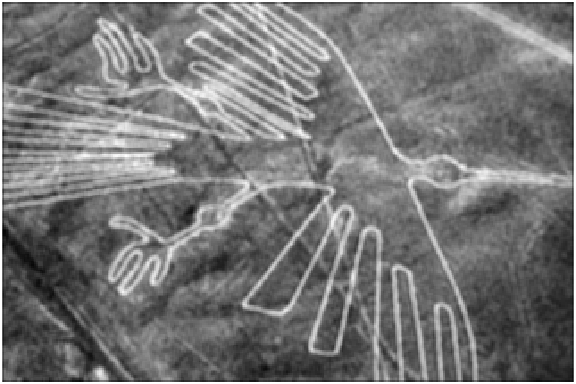
\includegraphics[width=0.8\textwidth]{smoothed_image.png}
    \caption{Smoothed Image using Moving Average Filter}
\end{figure}

\newpage
\section*{Problem 2: Smoothing Effect with Different Weights}
Composite images illustrating the smoothing effect with different weights are shown below:

\begin{figure}[H]
    \centering
    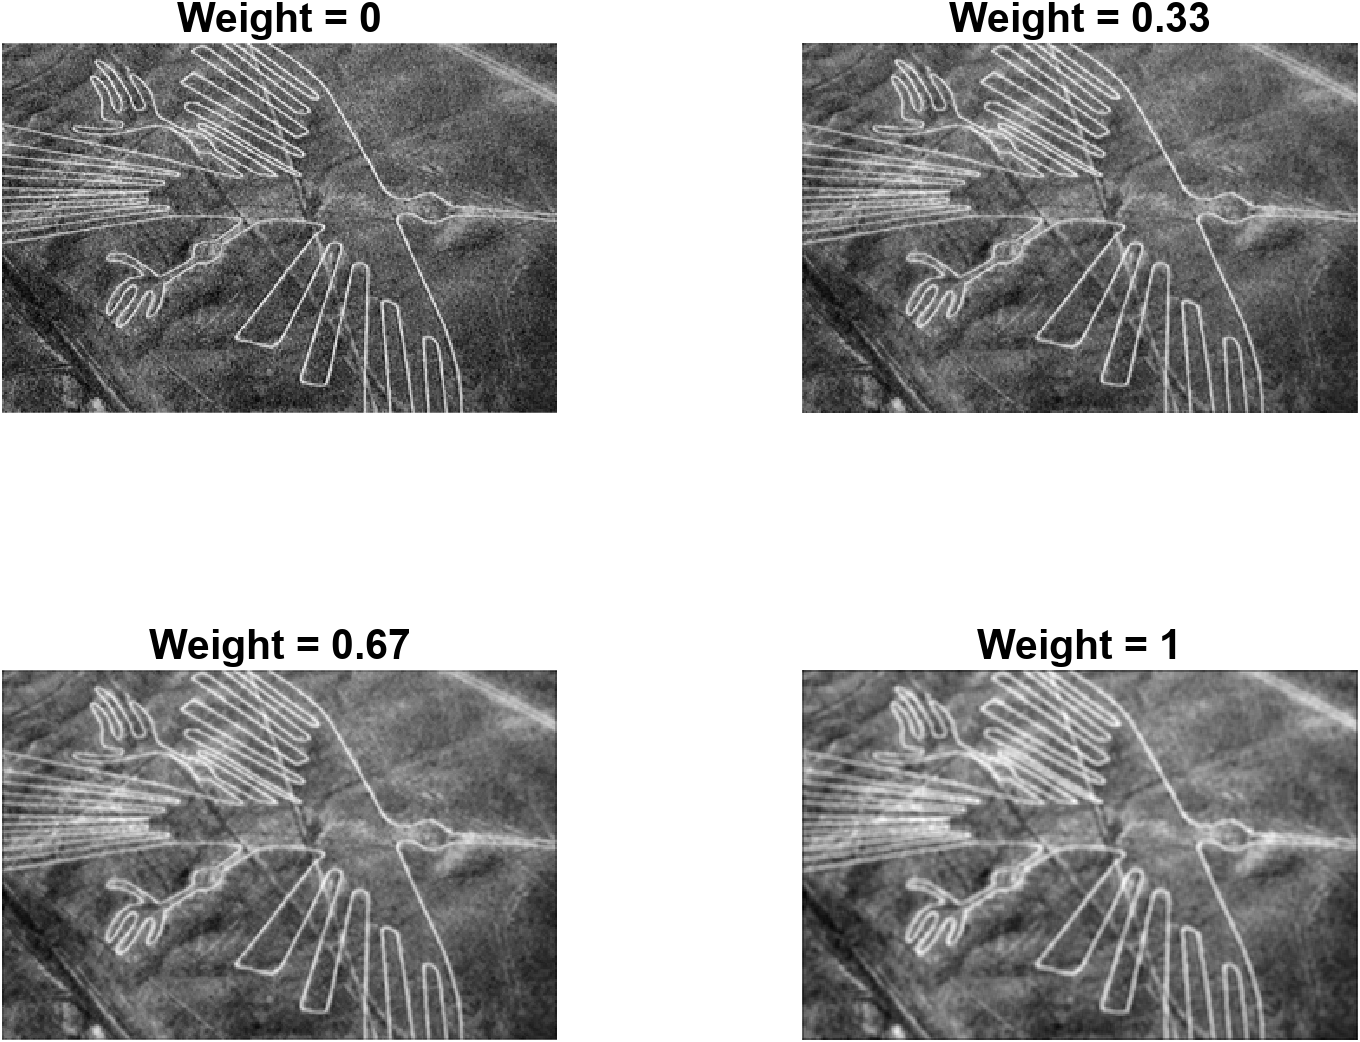
\includegraphics[width=0.9\textwidth]{smoothed_composites.png}
    \caption{Composite Images with Smoothing Effect}
\end{figure}

\newpage
\section*{Problem 3: Gradient Filter for Edge Detection}
The gradient filters for horizontal and vertical edge detection are defined as:
\[
\bm{H_x} = \begin{bmatrix}
-1 & 0 & 1 \\
-2 & 0 & 2 \\
-1 & 0 & 1
\end{bmatrix}, \quad
\bm{H_y} = \begin{bmatrix}
-1 & -2 & -1 \\
0 & 0 & 0 \\
1 & 2 & 1
\end{bmatrix}
\]
The combined gradient filter is:
\[
\bm{H_{combined}} = \begin{bmatrix}
-1 + j & 2j & 1 + j \\
-2 & 0 & 2 \\
-1 - j & -2j & 1 - j
\end{bmatrix}
\]

\vspace{1cm}
\noindent{The edge profiles obtained using these filters are shown below:}
\begin{figure}[H]
    \centering
    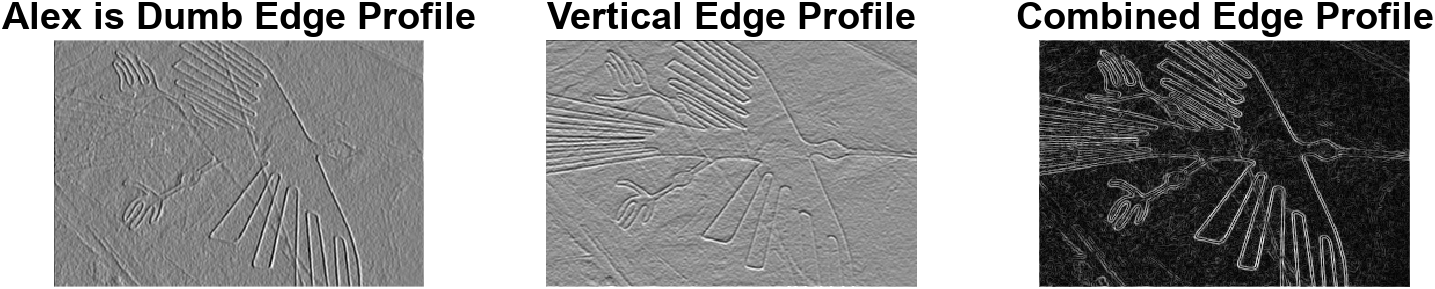
\includegraphics[width=1\textwidth]{edge_profiles.png}
    \caption{Edge Profiles: Horizontal, Vertical, and Combined}
\end{figure}


\newpage
\section*{Problem 4: Composite Images with Edge Detection}
Composite images illustrating the edge-detection effect are shown below:

\begin{figure}[H]
    \centering
    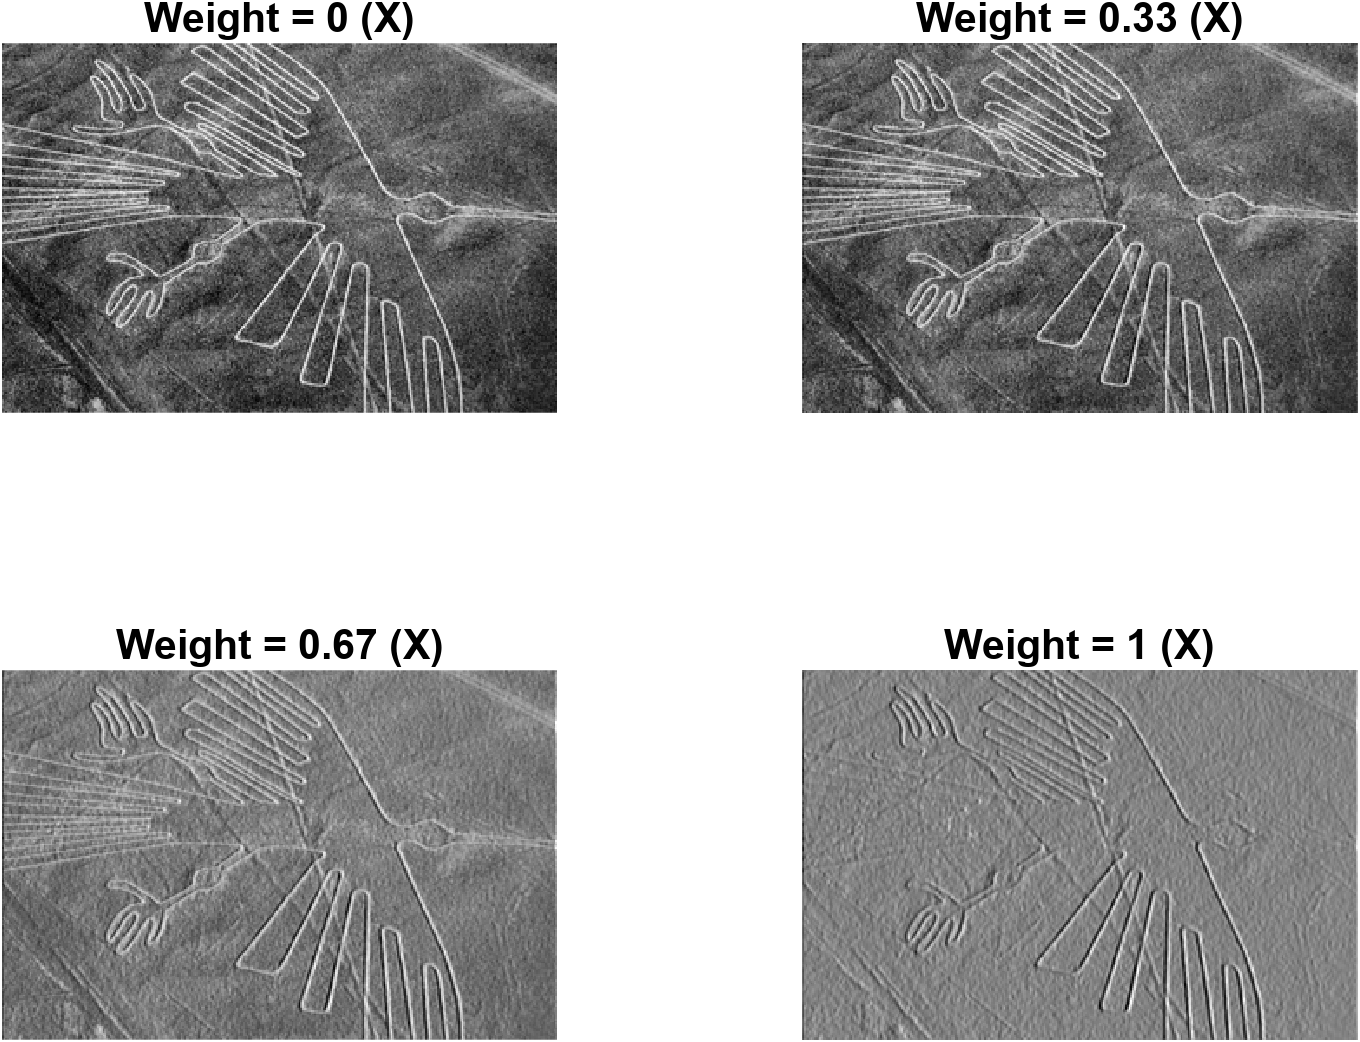
\includegraphics[width=0.9\textwidth]{horizontal_edge_composites.png}
    \caption{Composite Images with Horizontal Edge Detection}
\end{figure}

\vspace{1cm}
\begin{center}
    \textit{Continued below.}
\end{center}

\begin{figure}[H]
    \centering
    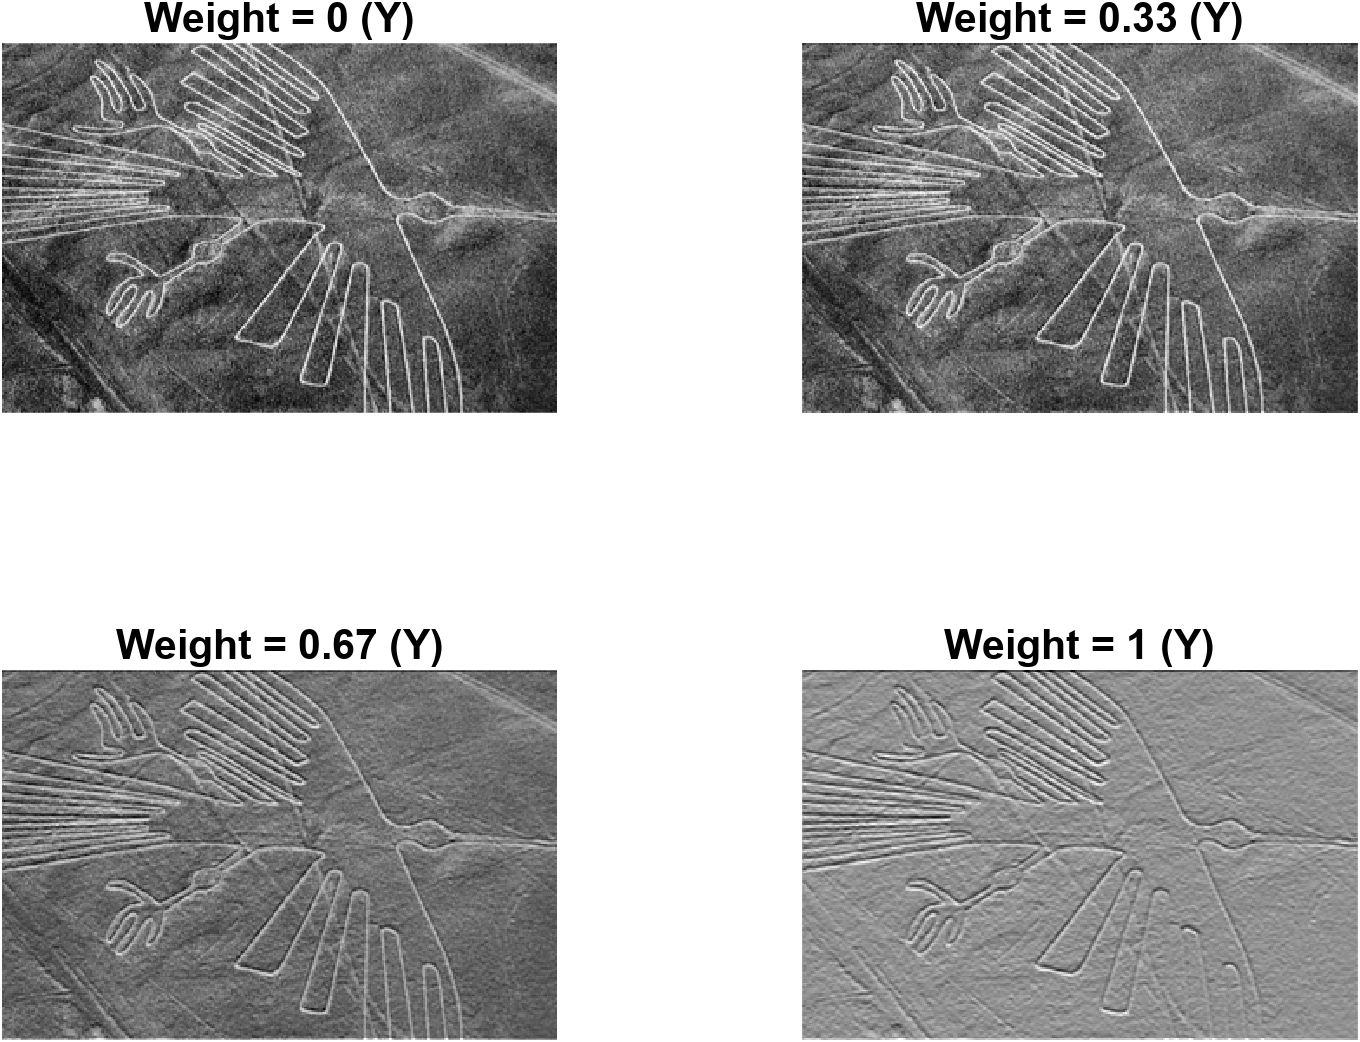
\includegraphics[width=0.75\textwidth]{vertical_edge_composites.png}
    \caption{Composite Images with Vertical Edge Detection}
\end{figure}

\begin{figure}[H]
    \centering
    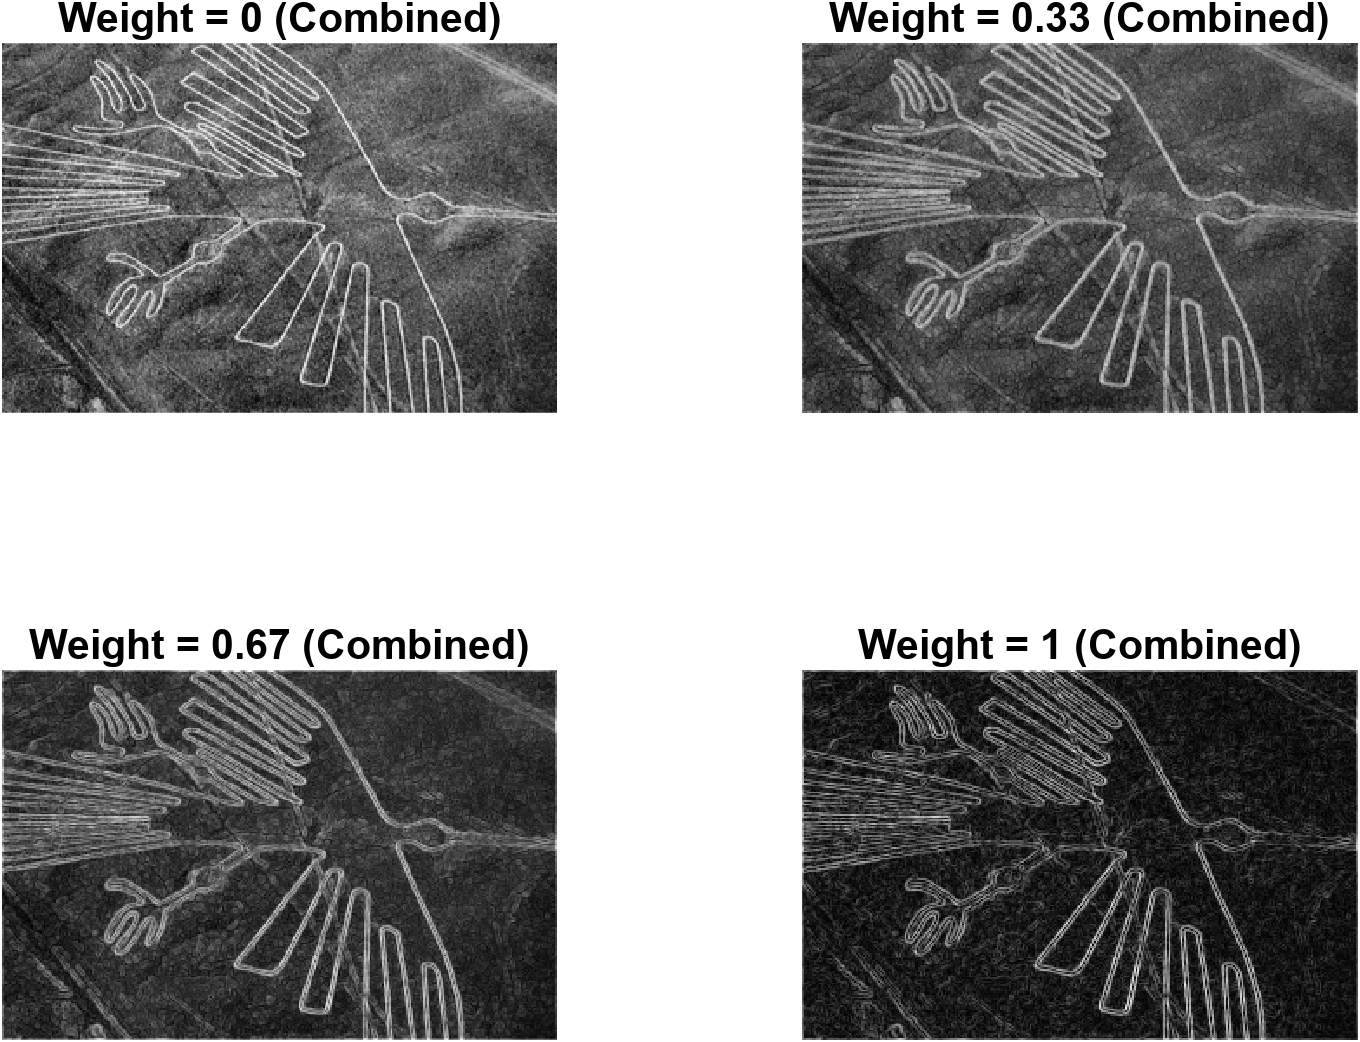
\includegraphics[width=0.75\textwidth]{combined_edge_composites.png}
    \caption{Composite Images with Combined Edge Detection}
\end{figure}


\newpage
\section*{Problem 5: Laplacian Filter for Peak Detection}
The Laplacian filter is defined as:
\[
\bm{H} = \begin{bmatrix}
0 & -1 & 0 \\
-1 & 4 & -1 \\
0 & -1 & 0
\end{bmatrix}
\]

\vspace{1cm}
The image obtained by applying the Laplacian filter for peak detection is shown below:

\begin{figure}[H]
    \centering
    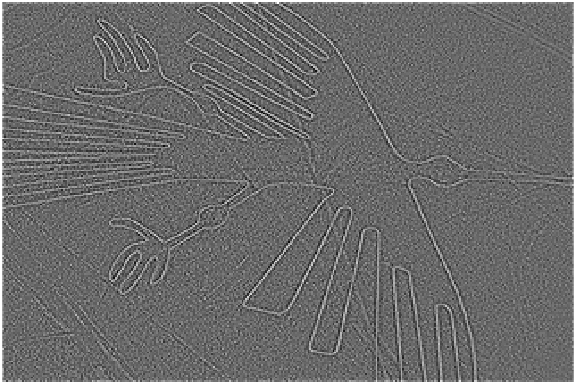
\includegraphics[width=0.75\textwidth]{laplacian_image.png}
    \caption{Laplacian Filtered Image for Peak Detection}
\end{figure}


\newpage
\section*{Problem 6: Composite Images with Peak Detection}
Composite images illustrating the peak-detection effect are shown below:

\begin{figure}[H]
    \centering
    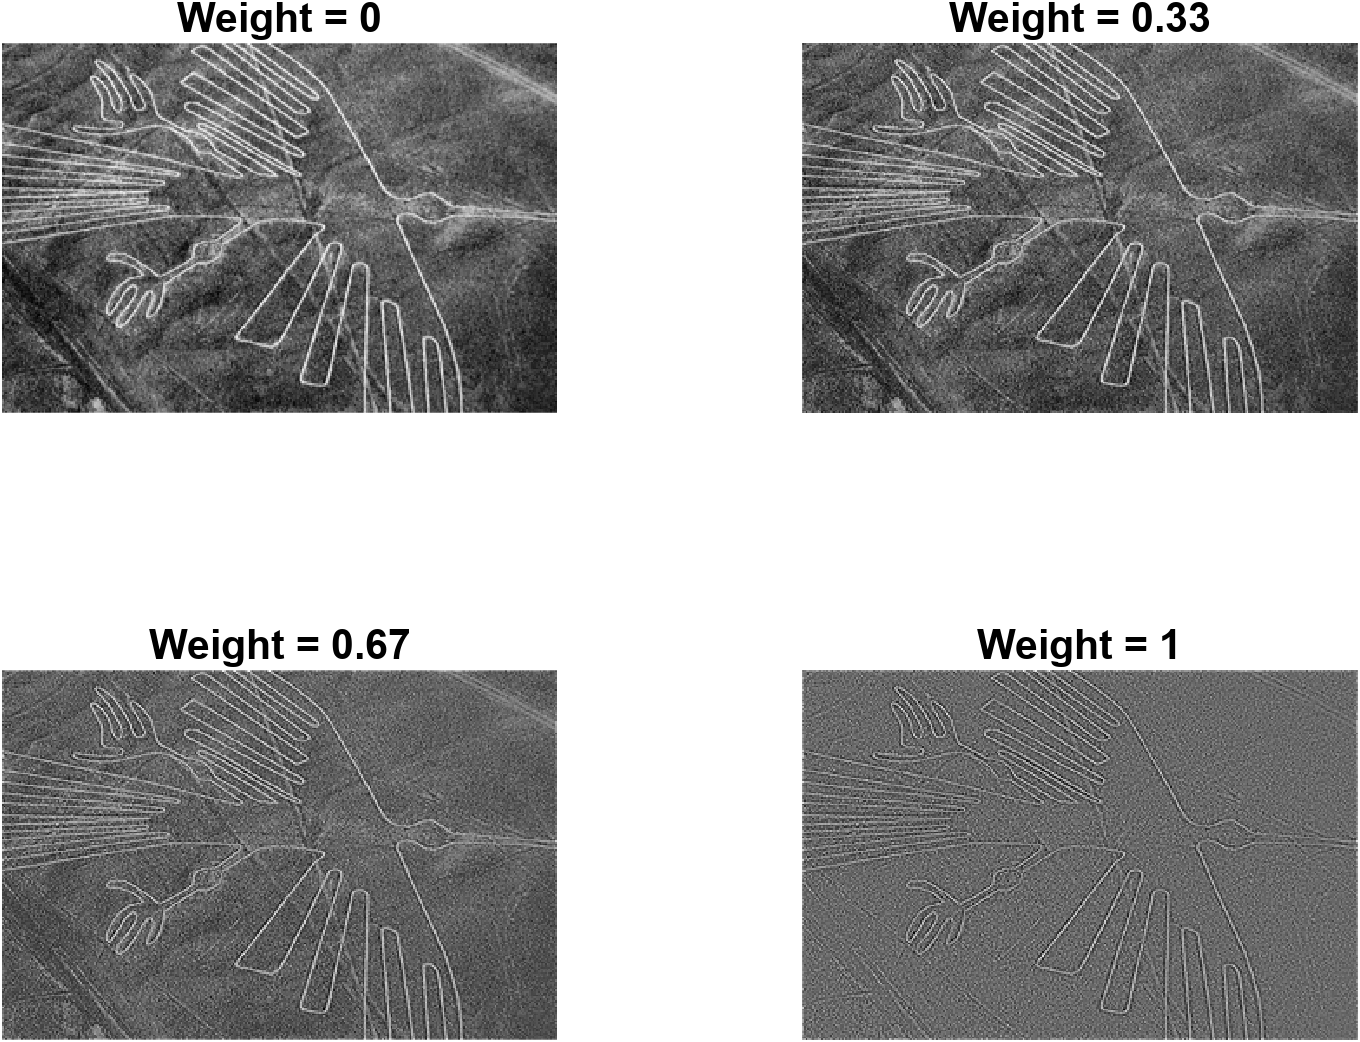
\includegraphics[width=0.9\textwidth]{laplacian_composite_images.png}
    \caption{Composite Images with Peak Detection Effect}
\end{figure}


\newpage
\section*{Summary}
\begin{itemize}
    \item The moving average filter effectively smooths the image, as shown in the smoothed image and composite results.
    \item A larger kernel filter would likely produce a more pronounced smoothing effect.
    \item The gradient filters successfully detect edges in horizontal, vertical, and combined directions, with clear edge profiles.
    \item The composite images demonstrate the edge-detection effect, with distinct edges highlighted.
    \item The combined gradient filter captures both horizontal and vertical edges, enhancing the edge-detection effect.
    \item This is especially apparent when you zoom in; one can perceive two distinct lines around the bird shape.
    \item The Laplacian filter highlights peaks in the image, and the composite images demonstrate the peak-detection effect.
    \item Interstingly, the Laplacian filter does not produce the contrast of the combined gradient filter, but it does produce a more pronounced peak-detection effect.
    \item There is no "two line" effect from the Laplacian filter; it's geared to bicked up the center of the lines.
\end{itemize}

\end{document}
